\begin{artengenv2auth}{Roman Krzanowski, Pawel Polak}
	{The meta-ontology of AI systems with human-level intelligence}
	{The meta-ontology of AI systems with human-level intelligence}
	{The meta-ontology of AI systems with human-level intelligence}
	{\textsuperscript{1}Departments of Philosophy and Mathematics, Carnegie Mellon University\\
		\textsuperscript{2}Copernicus Center for Interdisciplinary Studies, Jagiellonian University}
	{In this paper, we examine the meta-ontology of AI systems with human-level intelligence, with us denoting such AI systems as AI\textsubscript{E}. Meta-ontology in philosophy is a~discourse centered on ontology, ontological commitment, and the truth condition of ontological theories. We therefore discuss how meta-ontology is conceptualized for AI\textsubscript{E} systems. We posit that the meta-ontology of AI\textsubscript{E~}systems is not concerned with computational representations of reality in the form of structures, data constructs, or computational concepts, while the ontological commitment of AI\textsubscript{E} systems is directed toward what exists in the outside world. Furthermore, the truth condition of the ontology (which is meta-ontological assumption) of AI\textsubscript{E} systems does not require consistency with closed conceptual schema or ontological theories but rather with reality, or in other words, ``what is the world''
	%\label{ref:RNDuTcZpb4G1k}(Smith, 2019, p.57).
	\parencite[][p.57]{smith_promise_2019}. %
	 In addition, the truth condition of AI\textsubscript{E} systems is verified through operational success rather than by coherence with theories. This work builds on ontological postulates about AI systems that were formulated by Brian Caldwell Smith 
	%\label{ref:RND1W3b57kSJx}(2019).
	\parencite*[][]{smith_promise_2019}.%
	}
	{human-level intelligence AI, meta-ontology of AI Paradigm, AI Paradigm, ontology of AI Paradigm, ontological commitment of AI Paradigm, J. Haugeland, B. C. Smith, M. Minsky, H. Dreyfus.}
	{%
		{\flushright\subbold{Roman Krzanowski}\\\subsubsectit\small{Pontifical University of John Paul II in Krakow}\par}%
		{\flushright\subbold{Pawel Polak}\\\subsubsectit\small{Pontifical University of John Paul II in Krakow}\par}%
	}



%\begin{document}
%\title{The meta-ontology of AI systems with human-level intelligence}
%\maketitle
%
%\section{Abstract}
%In this paper, we examine the meta-ontology of AI systems with human-level intelligence, with us denoting such AI systems as AI\textsubscript{E}. Meta-ontology in philosophy is a~discourse centered on ontology, ontological commitment, and the truth condition of ontological theories. We therefore discuss how meta-ontology is conceptualized for AI\textsubscript{E} systems. We posit that the meta-ontology of AI\textsubscript{E~}systems is not concerned with computational representations of reality in the form of structures, data constructs, or computational concepts, while the ontological commitment of AI\textsubscript{E} systems is directed toward what exists in the outside world. Furthermore, the truth condition of the ontology (which is meta-ontological assumption) of AI\textsubscript{E} systems does not require consistency with closed conceptual schema or ontological theories but rather with reality, or in other words, ``what is the world''
%%\label{ref:RNDuTcZpb4G1k}(Smith, 2019, p.57).
%\parencite[][p.57]{smith_promise_2019}. %
% In addition, the truth condition of AI\textsubscript{E} systems is verified through operational success rather than by coherence with theories. This work builds on ontological postulates about AI systems that were formulated by Brian Caldwell Smith 
%%\label{ref:RND1W3b57kSJx}(2019).
%\parencite*[][]{smith_promise_2019}.%
%
%
%Keywords: \textit{human-level intelligence AI, meta-ontology of AI Paradigm, AI Paradigm, ontology of AI Paradigm, ontological commitment of AI Paradigm, J. Haugeland, B. C. Smith, M. Minsky, H. Dreyfus.}

\section{Introduction}
AI systems have developed over the past 60 years, bringing new solutions to a~huge number of practical problems, and they continue to find many surprising and fascinating applications. However, the main goal of AI, namely the creation of a~human-like intelligence, \footnotetext{See ft. 3 on AGI for an explanation of human-like intelligence.} is still proving unattainable. Indeed, the
AI systems we currently design and implement cannot replicate human intelligence and a~human agent's ability to cope with reality
%\label{ref:RNDzbUfjwINVD}(see e.g. Brooks, 1991; Minsky, 1991; Dreyfus, 2016; Mitchell, 2019; Bołtuć, 2020; Roitblat, 2020; Wooldridge, 2021).
\parencites[see, e.g.,][]{brooks_intelligence_1991}[][]{minsky_logical_1991}[][]{dreyfus_skillful_2016}[][]{mitchell_artificial_2019}[][]{boltuc_conscious_2020}[][]{roitblat_algorithms_2020}[][]{wooldridge_road_2021}.%


One of the reasons for this failing (in their ability to cope with reality) is, it seems, related to how these AI systems lack a~proper ontology or representation of the real world. (For more about the failings of current AI conceptualizations, see, for example, the works of Brooks
%\label{ref:RNDRn6fjQo5fK}(1991),
\parencite*[][]{brooks_intelligence_1991}, %
 Dreyfus 
%\label{ref:RNDQXX8Yv0mJq}(2016),
\parencite*[][]{dreyfus_skillful_2016}, %
 and Smith 
%\label{ref:RNDVD6ttaHRwZ}(2019)
\parencite*[][]{smith_promise_2019}%
).\footnote{To get a~sense of the ontologies (and meta-ontologies) of the real world in biological agents, consult Ed Yong's book \textit{An Immense World} 
%\label{ref:RNDQEaQIHeWBf}(Yong, 2022).
\parencite[][]{yong_immense_2022}. %
Interesting analysis of deep learning systems ontological commitments see
%(Šekrst and Skansi, 2022).
\parencite[][]{sekrst_machine_2022}.} %
Smith 
%\label{ref:RNDAN4wrT01Ck}(2019, p.44)
\parencite*[][p.44]{smith_promise_2019} %
 proposed four features that AI systems should possess if they are to mimic humans' ability to cope with the real world (i.e., have human-level intelligence). These systems, which we here refer to as AI\textsubscript{E} systems, should be embodied, embedded, extended, and enactive 
%\label{ref:RND7XiVNpc9Oj}(see also Käufer and Chemero, 2021).
\parencite[see also][]{kaufer_phenomenology_2021}. %
 While these features are not ontological per se, but they do imply a~commitment to some ontology. What the kind of ontology these four features would entail is a~meta-ontological question that we explore in this paper, thus furthering the ideas studied by Krzanowski and Polak 
%\label{ref:RNDbpbe9vUMPT}(2022).
\parencite*[][]{krzanowski_ontology_2022}.%


This paper is organized as follows: First, we define some basic concepts related to the meta-ontological discourse, namely ontology, specifically ontology of computing and AI systems, meta-ontology, ontological commitment, and truth conditions. As these concepts have many interpretations, we need precise definitions to ensure that the subsequent discussion will be understood as intended. Next, we explain the main postulates of meta-ontology for AI\textsubscript{E} systems, the topic of this work. In the conclusion, we discuss the inherent limitations of ontologies (which is a~meta-ontological problem) for artificial systems such as AI\textsubscript{E}, their inability to match human intelligence, and the potential prospects for AI\textsubscript{E}. (For more on the problems of ontology in AI systems see, for example, Haugeland
%\label{ref:RNDYBbHi2hgVs}(1985)
\parencite*[][]{haugeland_artificial_1985} %
 and Fjelland 
%\label{ref:RNDnEqrE2ShbQ}(2020)
\parencite*[][]{fjelland_why_2020}%
).

Three things should be borne in mind while reading this paper. First, AI systems with human-level intelligence are often referred to as AGI systems, but with many interpretations for this concept, we avoid using this term to prevent us from drifting into the debate about AGI.\footnote{See various references for different conceptualizations of AGI
%\label{ref:RNDlE6bxZSweV}(e.g. Mitchell, 2019, p.40; Fjelland, 2020);
\parencites[e.g.,][p.40]{mitchell_artificial_2019}[][]{fjelland_why_2020}; %
 general purpose, human-level intelligence 
%\label{ref:RNDTtFTF8X0Xa}(Marcus, 2022);
\parencite[][]{marcus_artificial_2022}; %
 the generic ability of a~machine to consciously perform any task that a~human can 
%\label{ref:RND1RaLeokAOz}(Kumpulainen and Terziyan, 2022);
\parencite[][]{swar_unified_2022}; %
 the intelligence of a~machine that is capable of understanding the world 
%\label{ref:RND3vayfssWih}(Skuza, 2020);
\parencite[][]{skuza_what_2020}; %
 the representation of generalized human cognitive abilities 
%\label{ref:RNDtYCoFCClKk}(Lutkevich, 2022);
\parencite[][]{lutkevich_what_2022}; %
 a~general-purpose capability, including the ability to broadly generalize to fundamentally new areas 
%\label{ref:RNDQOScPjMeEk}(Cassimatis, Bello and Langley, 2008);
\parencite[][]{cassimatis_ability_2008}; %
 and the capacity of an engineered system to display the same rough sort of general intelligence as humans 
%\label{ref:RNDbpu6DOErGB}(Goertzel, 2015).
\parencite[][]{goertzel_artificial_2015}. %
 Creating human-level intelligence was always the aim of AI research, as attested to by Yann LeCun's recent claim ``Getting machines to behave like humans and animals has been the quest of my life'' (reported in \emph{\textup{2022 MIT Technology Review }}\label{ref:RNDzntlMH5EtX}\emph{\textup{(Heikkil}}ä and Heaven, 2022)\emph{\textup{)}.}} Second, this is a~study of the meta-ontology of specific AI systems, i.e., AI\textsubscript{E}, meaning that the focus of the study is ontology of these AI systems rather than philosophical ontology. Philosophy forms the background of this discussion, but it is not its main objective. Third, we are not concerned with particular implementations of AI\textsubscript{E} systems, which is why we instead study the AI\textsubscript{E} system paradigm, which is the all-encompassing conceptual framework of AI\textsubscript{E} systems that supports multiple implementations. Thus, when we talk about an AI\textsubscript{E} system, we are referring to an AI\textsubscript{E} system paradigm rather than a~specific implementation. The concept of AI paradigm and its role in this study are explained later in the paper.

\section{Key grounding ideas}
\subsection{The ontology of AI}

Ontology can be thought as an empty buzzword or a~specific conceptual construct,\footnote{``We must be careful in reading [auth. any] philosophical works on ontology, when the author speaks of ‘ontology' without qualifications, not to confuse the intended sense of the world with any of the alternatives''
%\label{ref:RNDfLy5S3W893}(Jacquette, 2002, p.3).
\parencite[][p.3]{jacquette_ontology_2002}. %
 There is also a~confusion between ontology and metaphysics. Some authors see ontology as the ultimate study of reality 
%\label{ref:RNDvlH3CHHmmY}(e.g. Jacquette, 2002; Stróżewski, 2004, p.32, or Perzanowski, 2015),
\parencites[e.g.,][]{jacquette_ontology_2002}[][]{strozewski_ontologia_2004}[or][]{perzanowski_rozprawa_2015}, %
 and metaphysics as being ``after physics'', some others see ontology as a~part of metaphysics 
%\label{ref:RNDeDepxi7xRN}(see e.g. Van Inwagen, 2009).
\parencite[see e.g.][]{van_inwagen_metaphysics_2009}. %
 In AI literature because ontology takes on a~very concrete garb (of an engineering domain) metaphysics is a~rare term so the confusion is not so visible.} so we need to position the ontology of AI\textsubscript{E~}within the world of ontological theories and demonstrate, what it means in this discussion, how it relates to ``other'' ontologies in philosophy, computer science, and AI. Ontology in computer science and AI systems 
%\label{ref:RNDxG2UeatxFk}(e.g. Sánchez, Cavero and Martínez, 2007; as well Guarino and Giaretta, 1995; Guarino, Oberle and Staab, 2009; Swar, Khoriba and Belal, 2022)
\parencites[e.g.,][]{sharman_road_2007}[as well][]{guarino_ontologies_1995}[][]{guarino_what_2009}[][]{swar_unified_2022} %
 takes on different meanings to that of philosophy 
%\label{ref:RNDWOSOcJkOvq}(e.g. Jacquette, 2002; Stróżewski, 2004; Baker, 2007; Chalmers, Wasserman and Manley, 2009; Effingham, 2013; Berto and Plebani, 2015; Perzanowski, 2015; Thomasson, 2015; Hofweber, 2021).
\parencites[e.g.,][]{jacquette_ontology_2002}[][]{strozewski_ontologia_2004}[][]{baker_metaphysics_2007}[][]{chalmers_metametaphysics_2009}[][]{effingham_introduction_2013}[][]{berto_ontology_2015}[][]{perzanowski_rozprawa_2015}[][]{thomasson_ontology_2015}[][]{hofweber_logic_2021}.%
\footnote{Importing AI (or technical) aspects into philosophy brings with it a~touch of reality that philosophical considerations often lack. See also the comment by Jacquette on the relation between a~domain ontology and the domain itself 
%\label{ref:RNDY4CVeRGcfL}(Jacquette, 2002, p.5).
\parencite[][p.5]{jacquette_ontology_2002}.%
} The philosophical concepts of ontology, however, are fundamental to those used in specific applications 
%\label{ref:RNDFJ4JNj0TbG}(see the comments of Jacquette, 2002, p.XII).
\parencite[see the comments of][p.XII]{jacquette_ontology_2002}. %
 This is therefore where we begin.

In philosophy, ontology is the study of being as it is (i.e., ``what is''), so it is about ``being'' in the most general sense\footnote{The term ``being'' is used in the sense employed by the Ancient Greeks, Parmenides (opposite to The Unbeing), Aristotle (Being qua being), medieval scholars like Aquinas (the study of being qua being)
%\label{ref:RNDFR1vKzYSIx}(Kerr, 2022),
\parencite[][]{kerr_aquinas_2022}, %
 and some modern philosophers such as 
%\label{ref:RNDYFnNv0y86Z}(Jacquette, 2002; Stróżewski, 2004, p.32, or Perzanowski, 2015).
\parencites[][]{jacquette_ontology_2002}[][]{strozewski_ontologia_2004}[or][]{perzanowski_rozprawa_2015}. %
 This term is also sometimes written as Being meaning totality of what exist 
%\label{ref:RNDjNhA4sxPMl}(Kenny, 2012, p.160).
\parencite[][p.160]{kenny_new_2012}. %
 Many modern philosophies, scientists computer engineers infuse this term with many different meanings (see this paper for the examples) obfuscating the original Greek sense of \textit{onto-logia} -- the fundamental study of being, probably as too esoteric (i.e., metaphysical) for their tastes 
%\label{ref:RNDjJRKpH1qcI}(see also Kenny, 2012; Hofweber, 2021).
\parencites[see also][]{kenny_new_2012}[][]{hofweber_logic_2021}.%
}. More specifically, in its purely philosophical meaning, ontology is the study of the foundations of what exists, what is common and most general among it, and what its origins are 
%\label{ref:RNDfYYNHUcznT}(see e.g. Jacquette, 2002; Stróżewski, 2004, p.32)
\parencites[see, e.g.,][]{jacquette_ontology_2002}[][p.32]{strozewski_ontologia_2004} %
 Hereafter, we refer to this concept by a~boldface, capital ``O'' without a~subscript (i.e., \textbf{O}).

Ontology in philosophy may also refer to ``what exists'' in a~much more constrained, narrower, sense. This kind of ontology investigates existing, subject to a~definition for existence, objects and relations in the world, and we will refer to this ontology as O. Depending on the assumptions made, different types of objects and relations may be recognized by O~ontologies, because O~branches into many subdomains. Thus, many different perspectives have been developed for ontology
%\label{ref:RNDJ0HiQvGuma}(e.g. Quine, 1960; Jacquette, 2002; Stróżewski, 2004; Baker, 2007; Chalmers, Wasserman and Manley, 2009; Effingham, 2013; Ingarden, 2013; 2016; Berto and Plebani, 2015; Perzanowski, 2015; Thomasson, 2015; Hofweber, 2021);
\parencites*[e.g.,][]{quine_word_1960}[][]{jacquette_ontology_2002}[][]{strozewski_ontologia_2004}[][]{baker_metaphysics_2007}[][]{chalmers_metametaphysics_2009}[][]{effingham_introduction_2013}[][]{ingarden_controversy_2013}[][]{ingarden_controversy_2016}[][]{berto_ontology_2015}[][]{perzanowski_rozprawa_2015}[][]{thomasson_ontology_2015}[][]{hofweber_logic_2021}; %
 these differ in terms of extent, content, consistency, and accuracy, often responding to the specific needs of a~domain.

\textbf{In computational systems}, ontology can be defined as ``a specific vocabulary (dictionary) used to describe a~certain reality, plus a~set of explicit assumptions regarding the intended meaning of the vocabulary words''
%\label{ref:RNDAcXPc7BmPe}(see Guarino and Giaretta, 1995; Guarino, Oberle and Staab, 2009).
\parencites[see][]{guarino_ontologies_1995}[][]{guarino_what_2009}. %
 In this context, ontologymay also refer to ``a model of the structure of a~system'' 
%\label{ref:RNDi9mTVDxk3A}(Guarino, Oberle and Staab, 2009)
\parencite[][]{guarino_what_2009} %
 or ``a formal, explicit specification of a~shared conceptualization'' 
%\label{ref:RNDAqesK2fTKs}(Studer, Benjamins and Fensel, 1998).
\parencite[][]{studer_knowledge_1998}. %
 We also have computational ontologies, which often called engineering ontologies, that ``are machine-processable structures which represent particular domains of interest'' 
%\label{ref:RNDiOONhTuWRW}(Husáková and Bureš, 2020).
\parencite[][]{husakova_formal_2020}. %
 Ontology may also be used to refer to knowledge-based systems, databases, or AI systems that manage knowledge bases 
%\label{ref:RND7tN9yeZ52M}(see the discussions of Sharman, Kishore and Ramesh, 2007; Staab and Studer, 2009; Garbacz and Oliver Kutz, 2014; Husáková and Bureš, 2020).
\parencites[see the discussions of][]{sharman_ontologies_2007}[][]{staab_handbook_2009}[][]{garbacz_formal_2014}[][]{husakova_formal_2020}.%


\textbf{The ontology of} AI\textsubscript{E} systems, meanwhile, denotes and determines how an AI\textsubscript{E} system represents and reasons about the real world. Itis not concerned with computational representations of reality through structures, theories, data constructs, or computational concepts but rather with how real world objects, properties, and relations are registered by an AI system, as well as how they are recognized and interpreted. In brief, this ontology is solely committed to the real world
%\label{ref:RNDHoOzRM31HN}(in the sense explained by Smith, 2019, p.145),
\parencite[in the sense explained by][p.145]{smith_promise_2019}, %
 with it reflecting the real world\footnote{The term ``real world'', or reality, is understood here as it is understood in Smith 
%\label{ref:RNDdF84GECegW}(2019, pp.xiii, xiv),
\parencite*[][xiv]{smith_promise_2019}, %
 denoting the physical world we live in. Minsky 
%\label{ref:RND166uXGx81U}(1991, p.6)
\parencite*[][p.6]{minsky_logical_1991} %
 refers to this reality as common sense reality. The term may be opposed to ``virtual worlds'', ``imaginary worlds'', ``fantastic worlds'', or other qualified uses of ``words'' denoting worlds as creations of computer systems, artistic expressions, or imaginations. The term ``world'' or ``real world'' may have multiple interpretations that we have no intention to discuss as such a~discussion would be pointless and would not further the main point of the paper. Thus, the reader seeking more detailed explanation of this term should follow the cited references..}, or physical reality, and the AI system's place in this world. More specifically, it is embodied, embedded, extended, and enactive 
%\label{ref:RNDcx3KAaKj2v}(Smith, 2019, p.43),
\parencite[][p.43]{smith_promise_2019}, %
 which are terms that will be explained later in this paper. There is no formal theory to accompany 4E ontology (ontology of AI system that is embodied, embedded, extended, and enactive), so there are no criteria for theoretical truth verification, but verification comes instead from a~confrontation with the real world, which we will discuss later. A~4E ontology is not given in the form of a~set of a~priori relations and objects but rather acquired 
%\label{ref:RNDIdA3C5UrQl}(Smith, 2019)
\parencite[][]{smith_promise_2019} %
 in response to a~dynamically changing reality 
%\label{ref:RNDjzZunSO8Xh}(see Minsky, 1991, as well as; Bołtuć, 2020).
\parencites[see][as well as]{minsky_logical_1991}[][]{boltuc_conscious_2020}. %
 We will refer to this ontology as O\textsubscript{E}.

Let us now put these things together. Ontology (\textbf{O}), as a~philosophical discipline, asks what is, in a~most general sense, and what exists Ontology (O) is more restricted with the scope of this ontology being defined by the horizon of interest: For example, it may be the universe, some aspect of it, or a~domain of reality (i.e., domain ontology), like ontology of biology, or ontology of physics. Ontology in computational systems, meanwhile, can be defined as ``a specific vocabulary used to describe a~certain reality, plus a~set of explicit assumptions regarding the intended meaning of the vocabulary entries,'' while the ontology of AI systems relates specifically to a~representation of the world or some knowledge domain in AI systems. Finally, the ontology of an AI\textsubscript{E} system (O\textsubscript{E}) refers to how AI\textsubscript{E} system represents about the real world and how it is situated within reality.

Figure \ref{krz-ill1} illustrates these ontological dependencies by showing them in terms of their increased specificity both in scope as well as in application domain, from the most general (\textbf{O}), which is the ontology of what exists (O), to the most specific one, which in this case is O\textsubscript{E}, the ontology of an AI\textsubscript{E} system.



%\begin{figure}[htp]
%\centering
%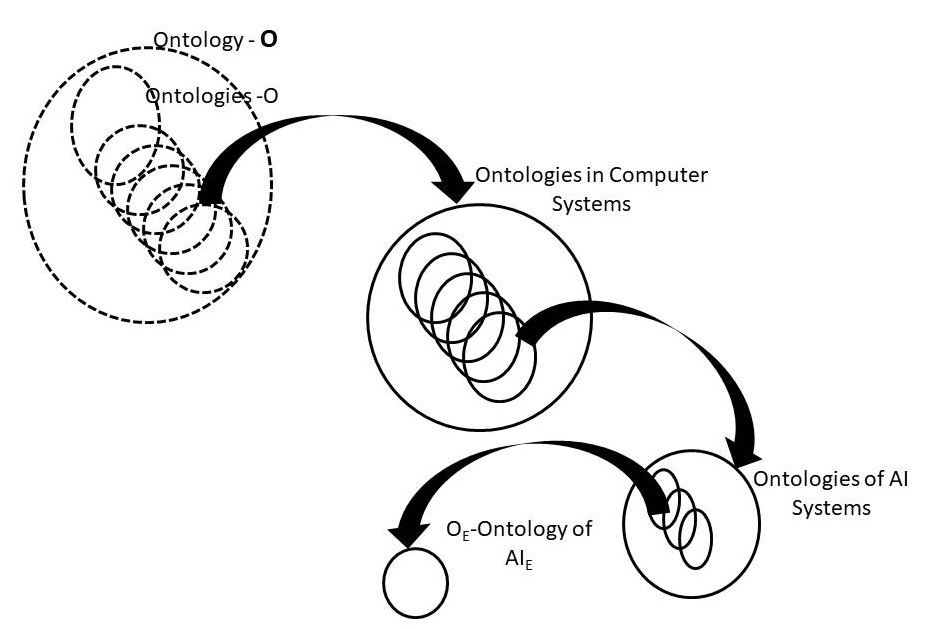
\includegraphics{ART_Krzanowski_Polak/Ontology2200B_pu.jpg}
%\end{figure}
%Figure 1. AI\textsubscript{E} ontology and hierarchy of ontologies.

\begin{figure}[htp]
 \begin{center}
 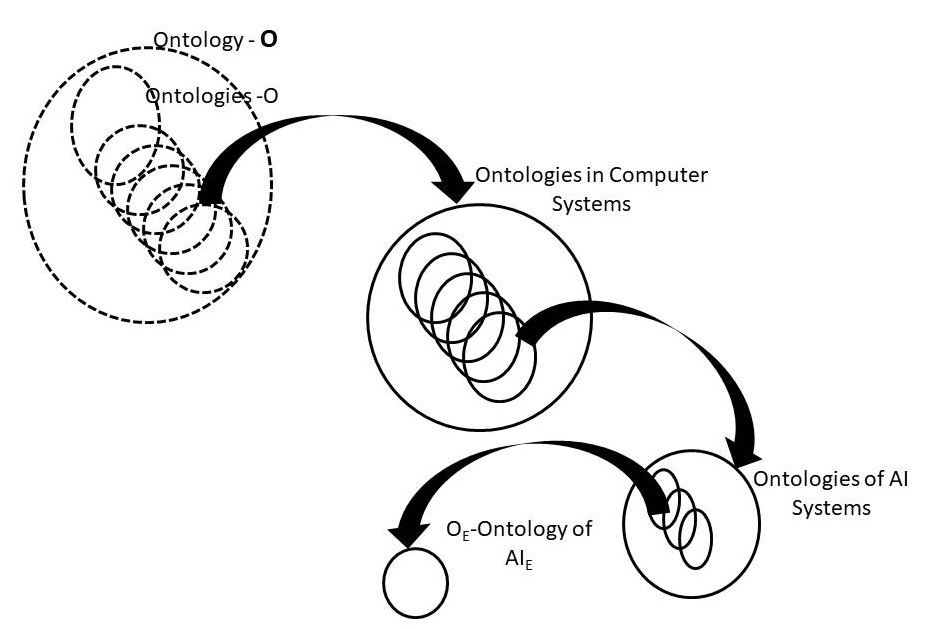
\includegraphics[width=.9\textwidth]{ART_Krzanowski_Polak/Ontology2200B_pu.jpg}%
 \end{center}%
 \caption{AI\textsubscript{E} ontology and hierarchy of ontologies.}\label{krz-ill1}
\end{figure}


Thus, with respect to specificity and scope, O\textsubscript{E} falls under the AI ontologies, which in turn are subspecies of the ontologies of computer systems, and these in turn are forms of specific ontologies (O) concerned with a~specific segment of reality, which then falls under fundamental ontology (\textbf{O}) for existence. All these ontologies ask the same question but within different contexts, scopes, and perspectives. Furthermore, Figure \ref{krz-ill1} shows how only ontology \textbf{O} attempts to comprehend all that exists, with other ontologies being mere fragments. The further away we move from the fundamental ontology \textbf{O}, the narrower and more specific the scope of the ontology becomes.

Thus, ontology that represents the real world being always expressed in some form of language (which always is) is always incomplete with respect to the world, i.e., the world ``as is'' cannot be represented by something else, despite the close isomorphism between the reality and some logical aka ontological systems \footnote{All pure ontological systems are logical systems
%\label{ref:RNDQXsIfZlLYA}(Jacquette, 2002, p.xiii; see e.g. Foschini, 2013).
\parencites[][p.xiii]{jacquette_ontology_2002}[see, e.g.,][]{foschini_where_2013}.%
}


\end{artengenv2auth}